\subsection{System description}
%The system can be described as a Classroom Response System (CRS) in the sense that it's a system made for polling and gathering responses in a classroom.

CRSFIT basically consists of rooms, groups, questions and answers, where users are able to ask questions, and gather responses.

A room is a collection of groups, and any user can create a room. The use of the term \emph{room} could be resembled with a classroom. It is possible to subscribe to a room, which makes it appear on the dashboard for easy access. The dashboard is the first thing you see when you log in and contains an overview of all rooms subscribed to and created. You may search for any room by using the search field in the menu bar. A blank search will show you every room available, and you may subscribe directly from the search results. It is also possible to simply obtain the rooms URL, and subscribe to it from there.

Within a room you'll find groups which is a collection of questions (hence a group). These groups are included in order to structure questions. There could be multiple reasons to why you would group questions together. One could be that you would want to make a group of questions public at once. Another reason could be that you would like to keep questions from each lecture separated in groups.

In order to control which groups and questions are open for answers, we made a feature that would let the owner control the access. This is done by pressing open/close on groups and questions. See figure \ref{fig:group} for a list of questions where some questions are open for answers while others har closed. This is indicated in the column \emph{Open for answers}. Subscribers of a room will be able to see closed groups but not the belonging questions. If a group is open, subscribers will be able to see the question but not answering them unless the questions are open as well. When clicking the \emph{Show info} button a small box with info about the particular question will be showed, as in figure \ref{fig:modal}. The box shows information about amount of answer options, received answers, how many students answered correct (in \% and only if the question is closed), when the question was created and when it was last changed.

\begin{figure}[H]
\capstart
	\centering
		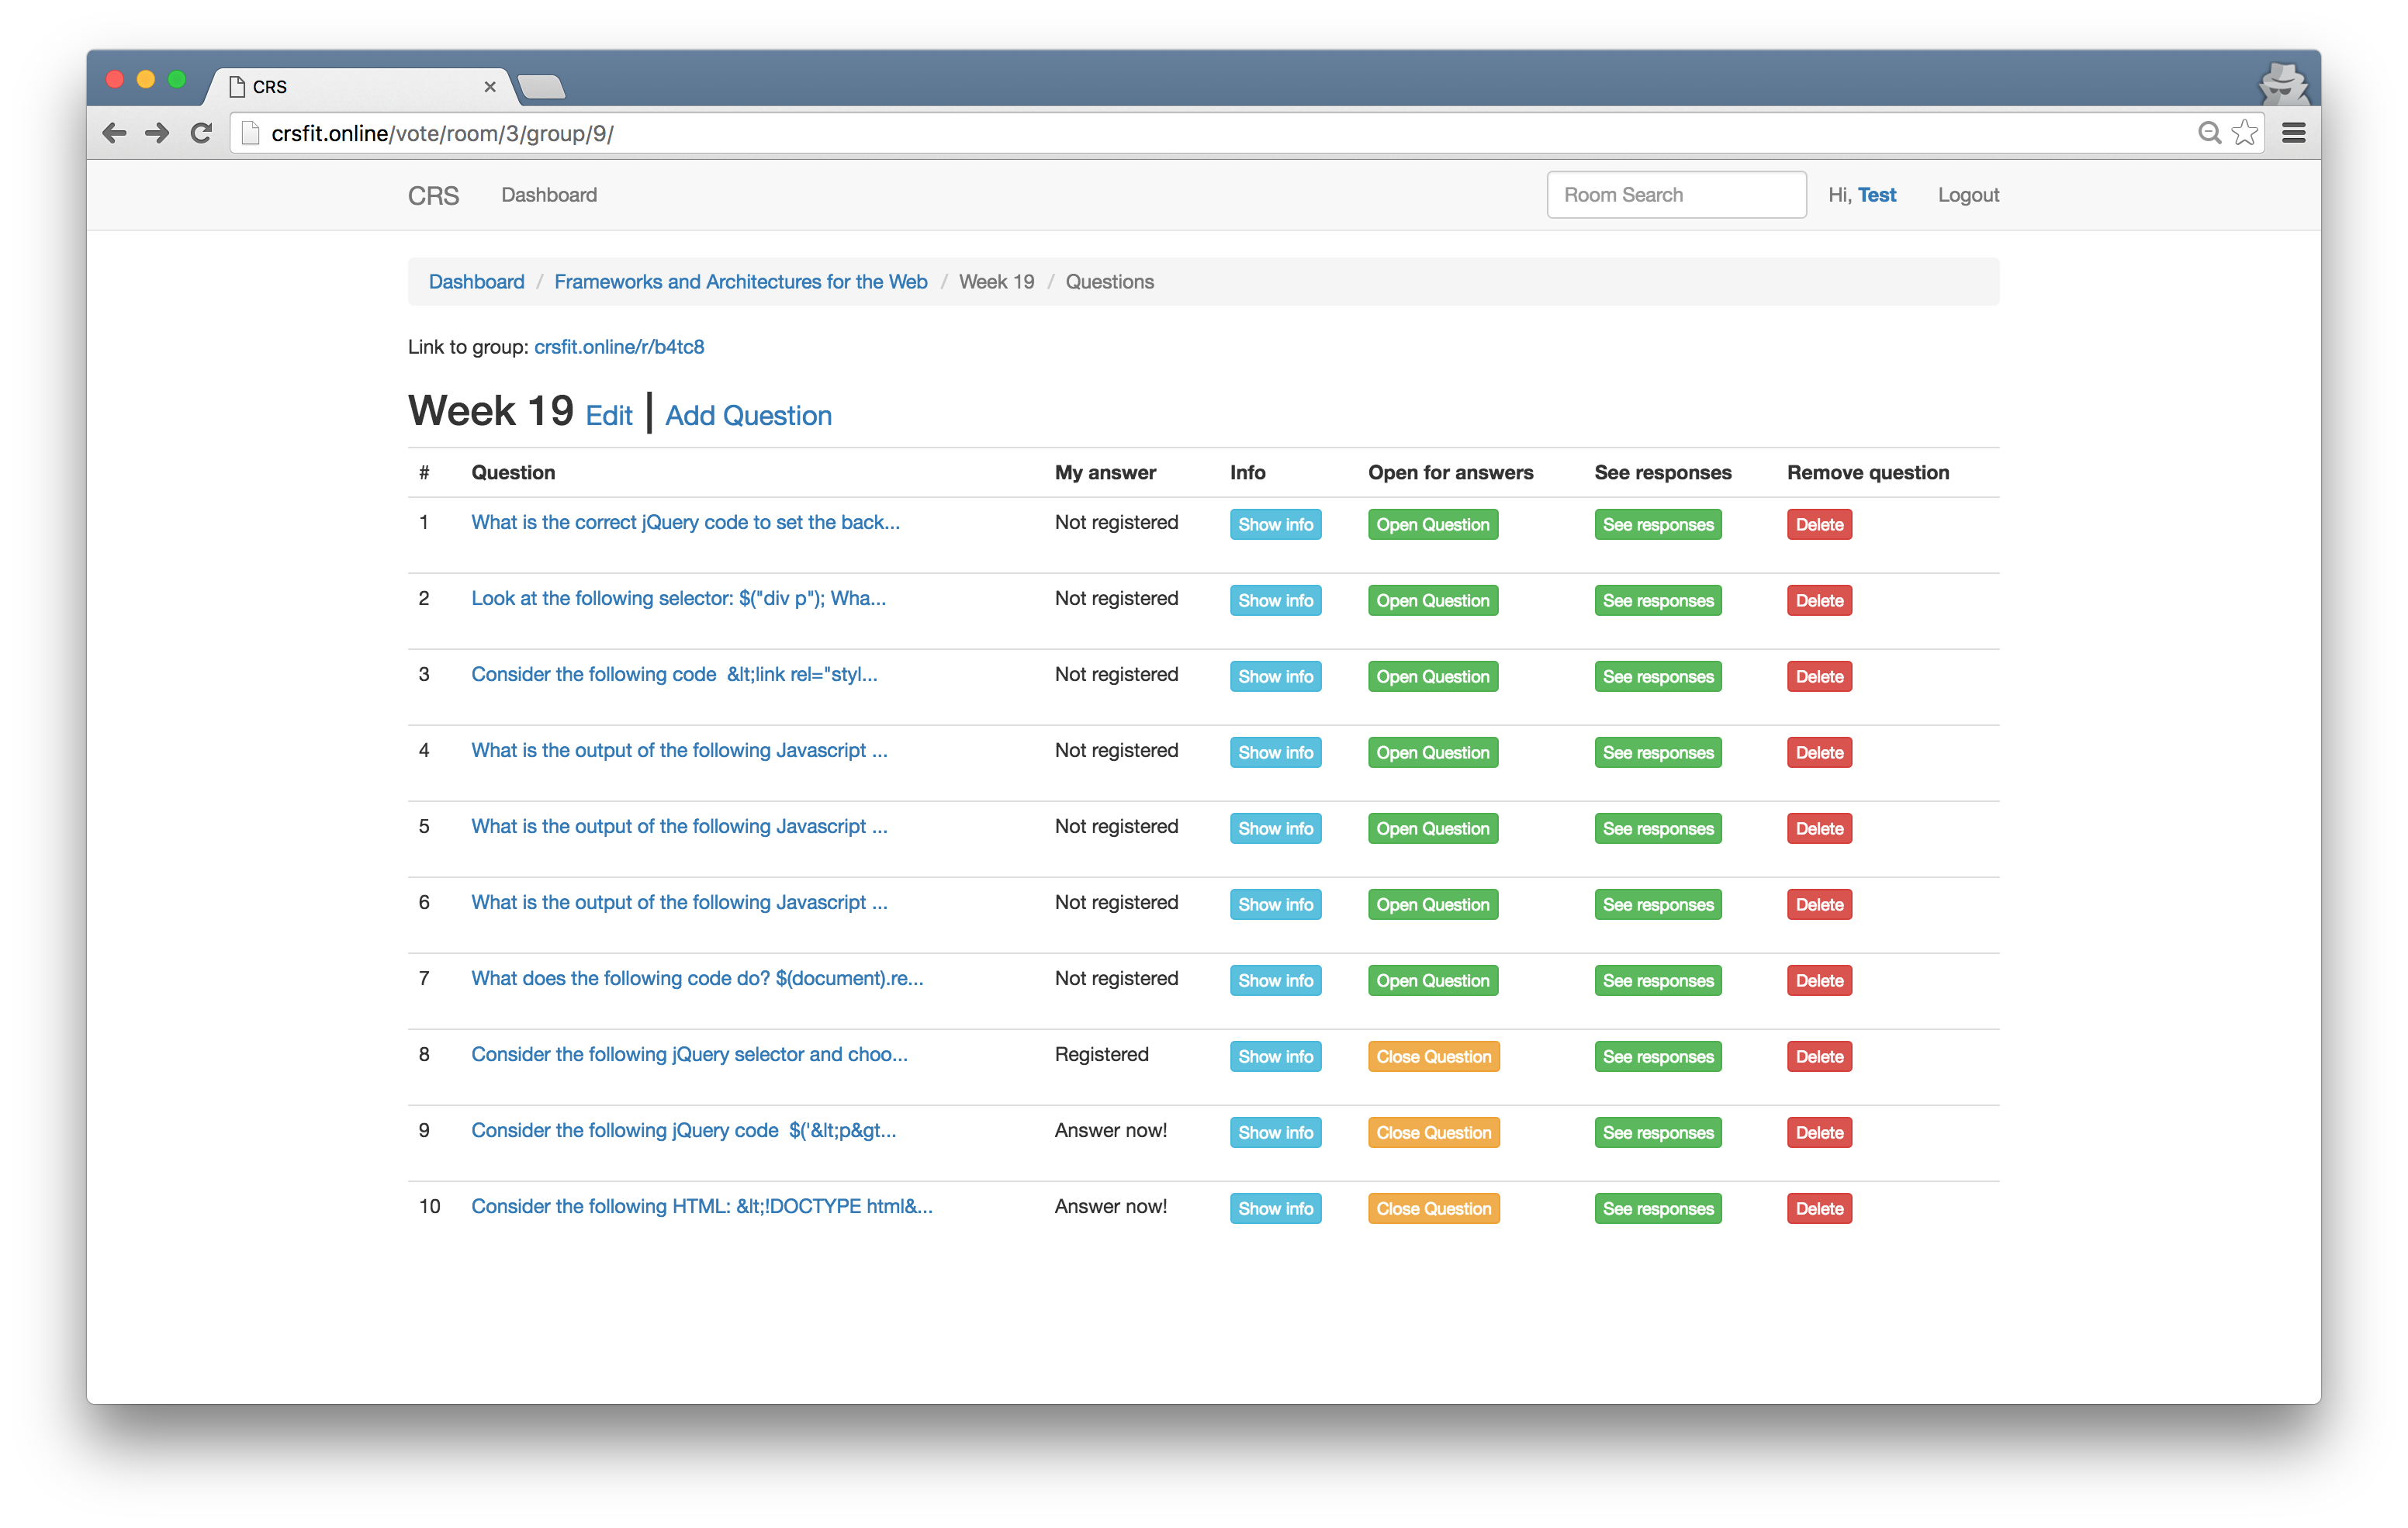
\includegraphics[width=\textwidth]{group.png}
	\caption[Inside a group]{A list of questions inside a group. The bottom three questions can be answered while the rest is currently closed.}\label{fig:group}
\end{figure}

\begin{figure}[H]
\capstart
	\centering
		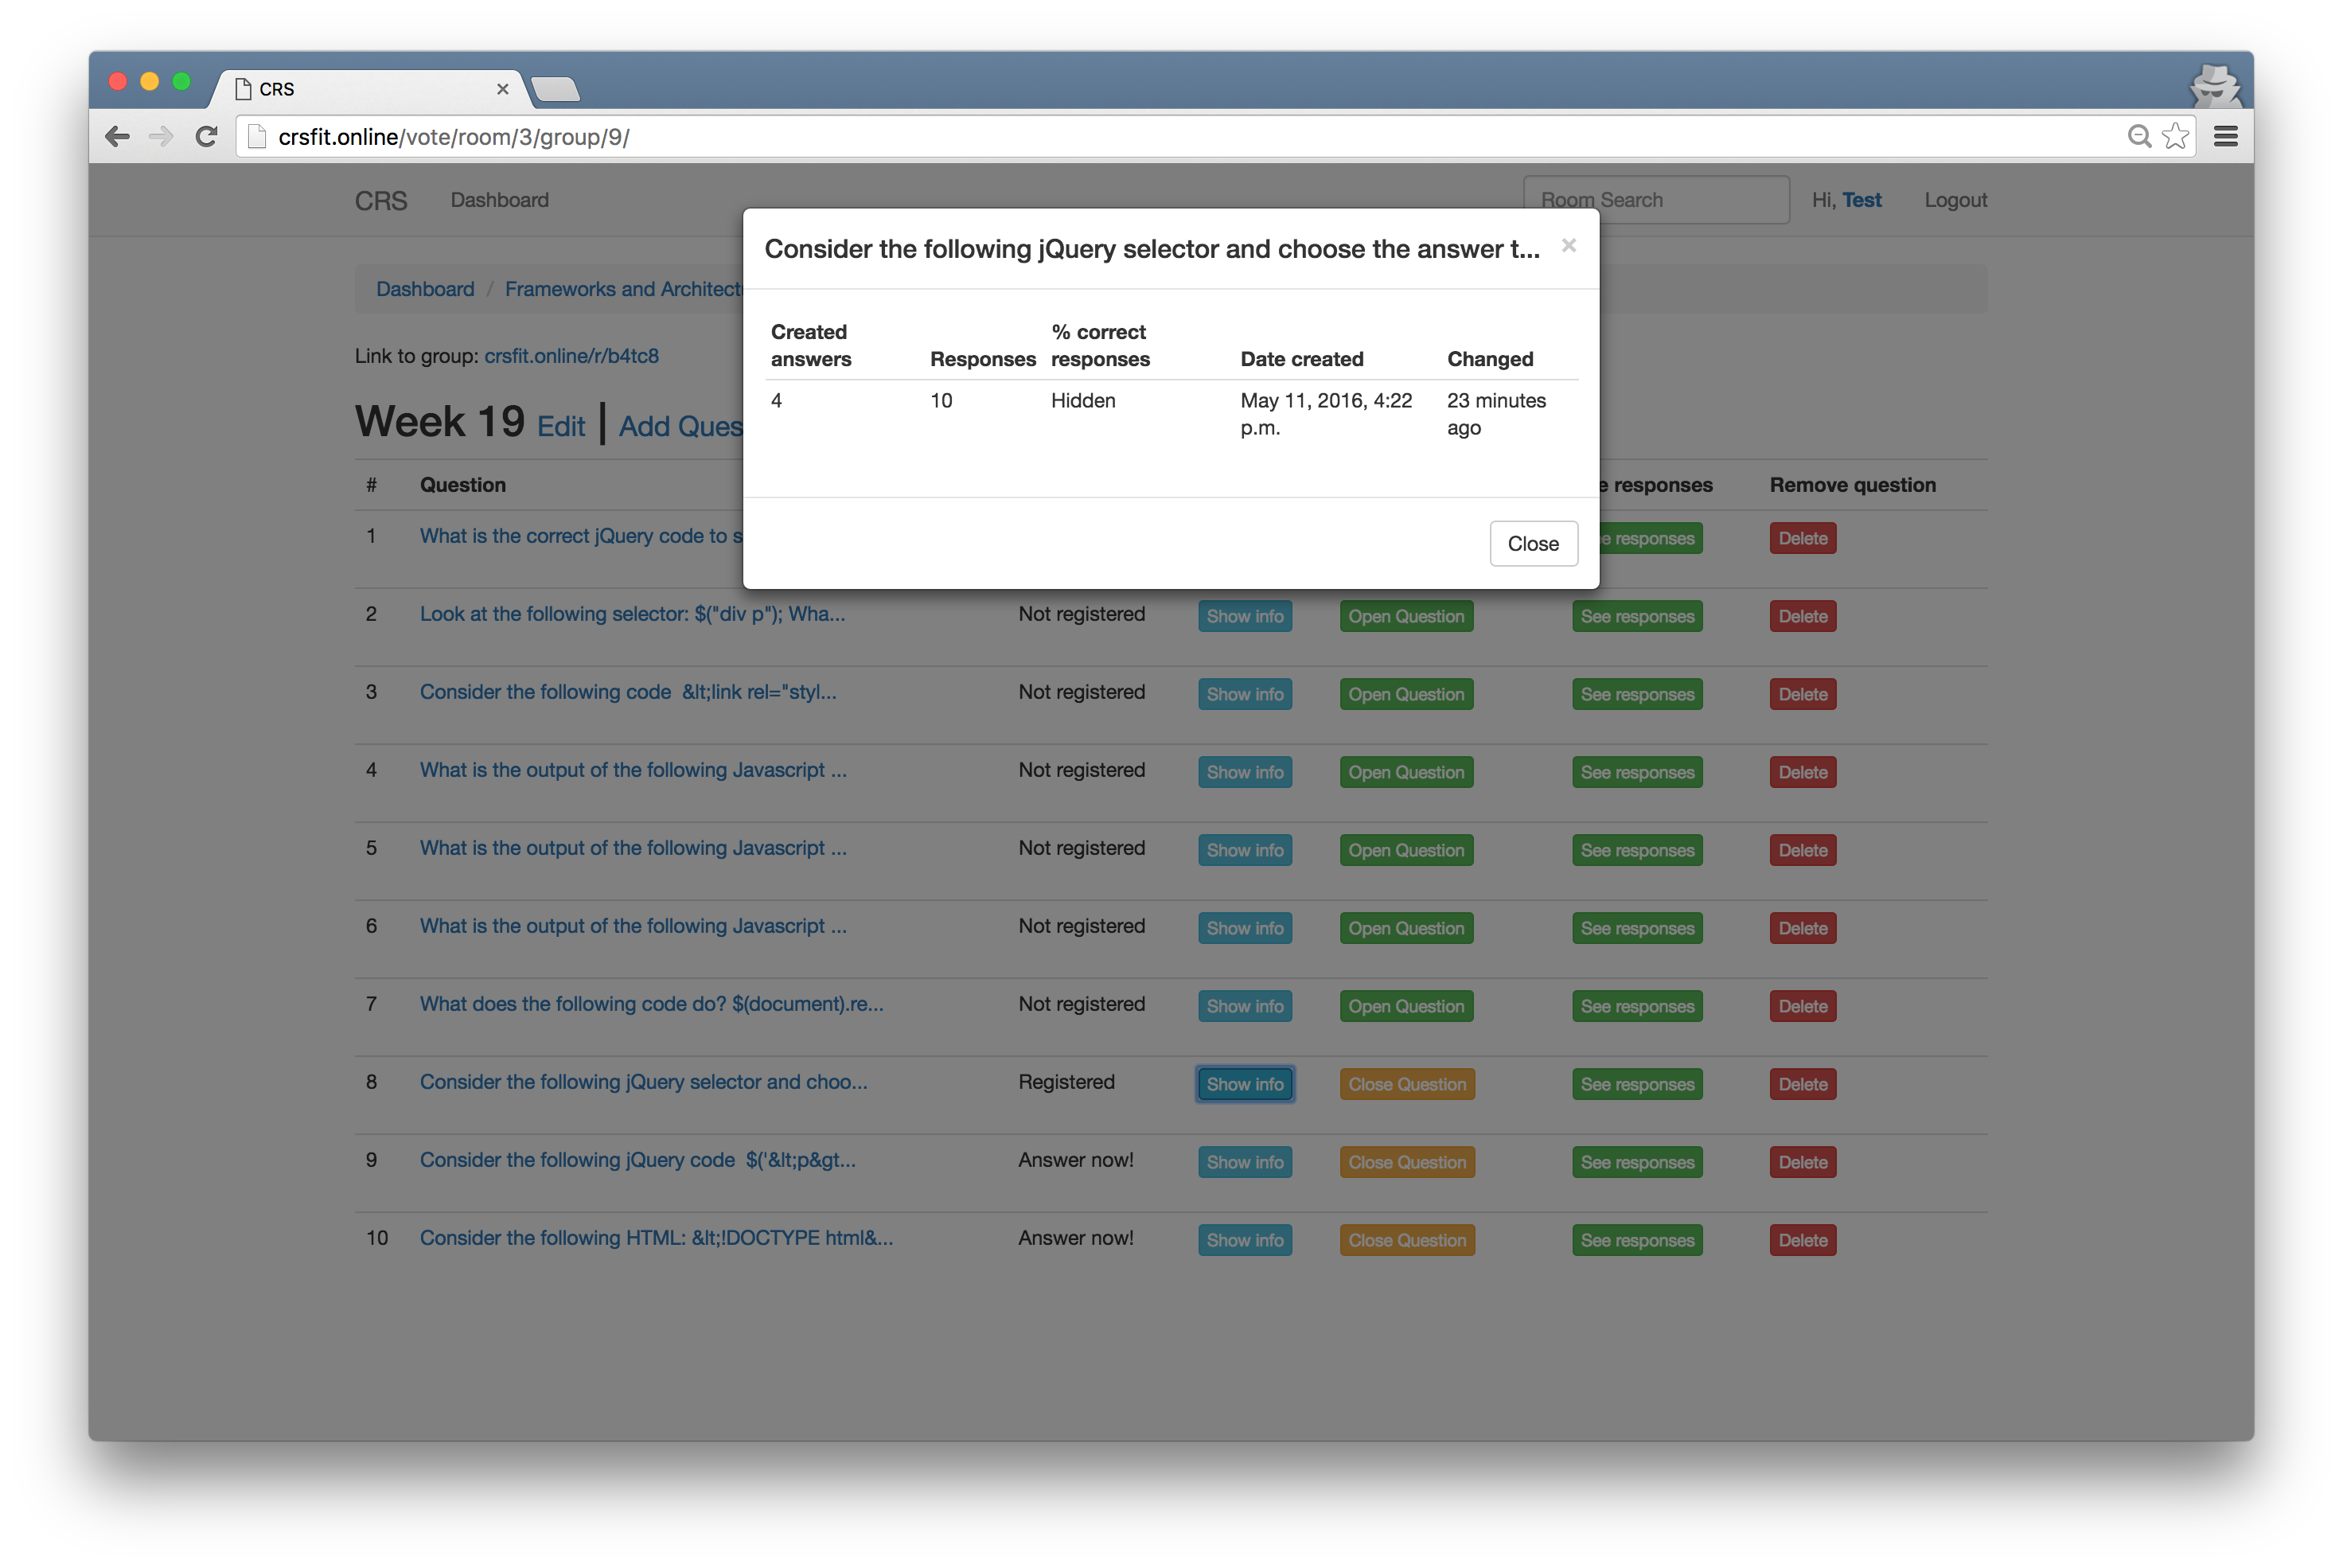
\includegraphics[width=\textwidth]{modal.png}
	\caption[Info box]{A box with info about a particular question.}\label{fig:modal}
\end{figure}

%% Main features
The main feature of the system consists of creating and answering questions. When you create a new question, you are presented with an option to create one or more answers.
These features are almost identical in every similar response system, and is part of the definition of the basic functionalities in a CRS. The structure as described above can be seen in figure \ref{fig:structure}.

\begin{figure}[H]
\capstart
	\centering
		\includegraphics[width=3.5cm]{structure.png}
	\caption[System Structure]{The system structure}\label{fig:structure}
\end{figure}

When creating and editing questions, we have made it possible to include code and mathematical expression in questions and answers. Code will be nicely formatted with the Prettify library \cite{google/code-prettify_2016} and mathematical expressions will be shown with the MathJax library \cite{mathjax_2016}. This eliminates the need for using different systems to ask questions when you want to include code or math. 

To show code, it is necessary to add \texttt{<pre>} tags around the code to add line numbers and syntax highlighting. We have added a convenient button to do this, so the user does not need to do it manually. The Prettify-library will automatically determine the language and highlight it accordingly. When writing mathematical expressions into a question or answer, the user will have to use the same syntax as in \LaTeX. This means that an expressions like \verb|$$a \ne 0$$| would be translated into $a \ne 0$ and \verb|$$x = {-b \pm \sqrt{b^2-4ac} \over 2a}$$| would be 
$$x = {-b \pm \sqrt{b^2-4ac} \over 2a}$$
This is meant to be convenient for people already knowing and using \LaTeX.

In theory, the system supports adding unlimited answers to a question. The only criteria is that an answer can't be left empty by the user. The creator of a question have the ability to mark one or more answers as correct. This will make subscribers able to track their performance and see whether they answered correctly or not. It's also possible not to mark an answer as correct if the system is simply used for polling, and there are no correct answer.

When responses are received to a question, the owner can track what is being answered in real time. See figure \ref{fig:responses} for a view of the response page. When enough responses are received, the owner can then close the question and the subscribers will be able to see the responses as well. Responses are shown with a chart which describes how many have chosen each answer.

\begin{figure}[H]
\capstart
	\centering
		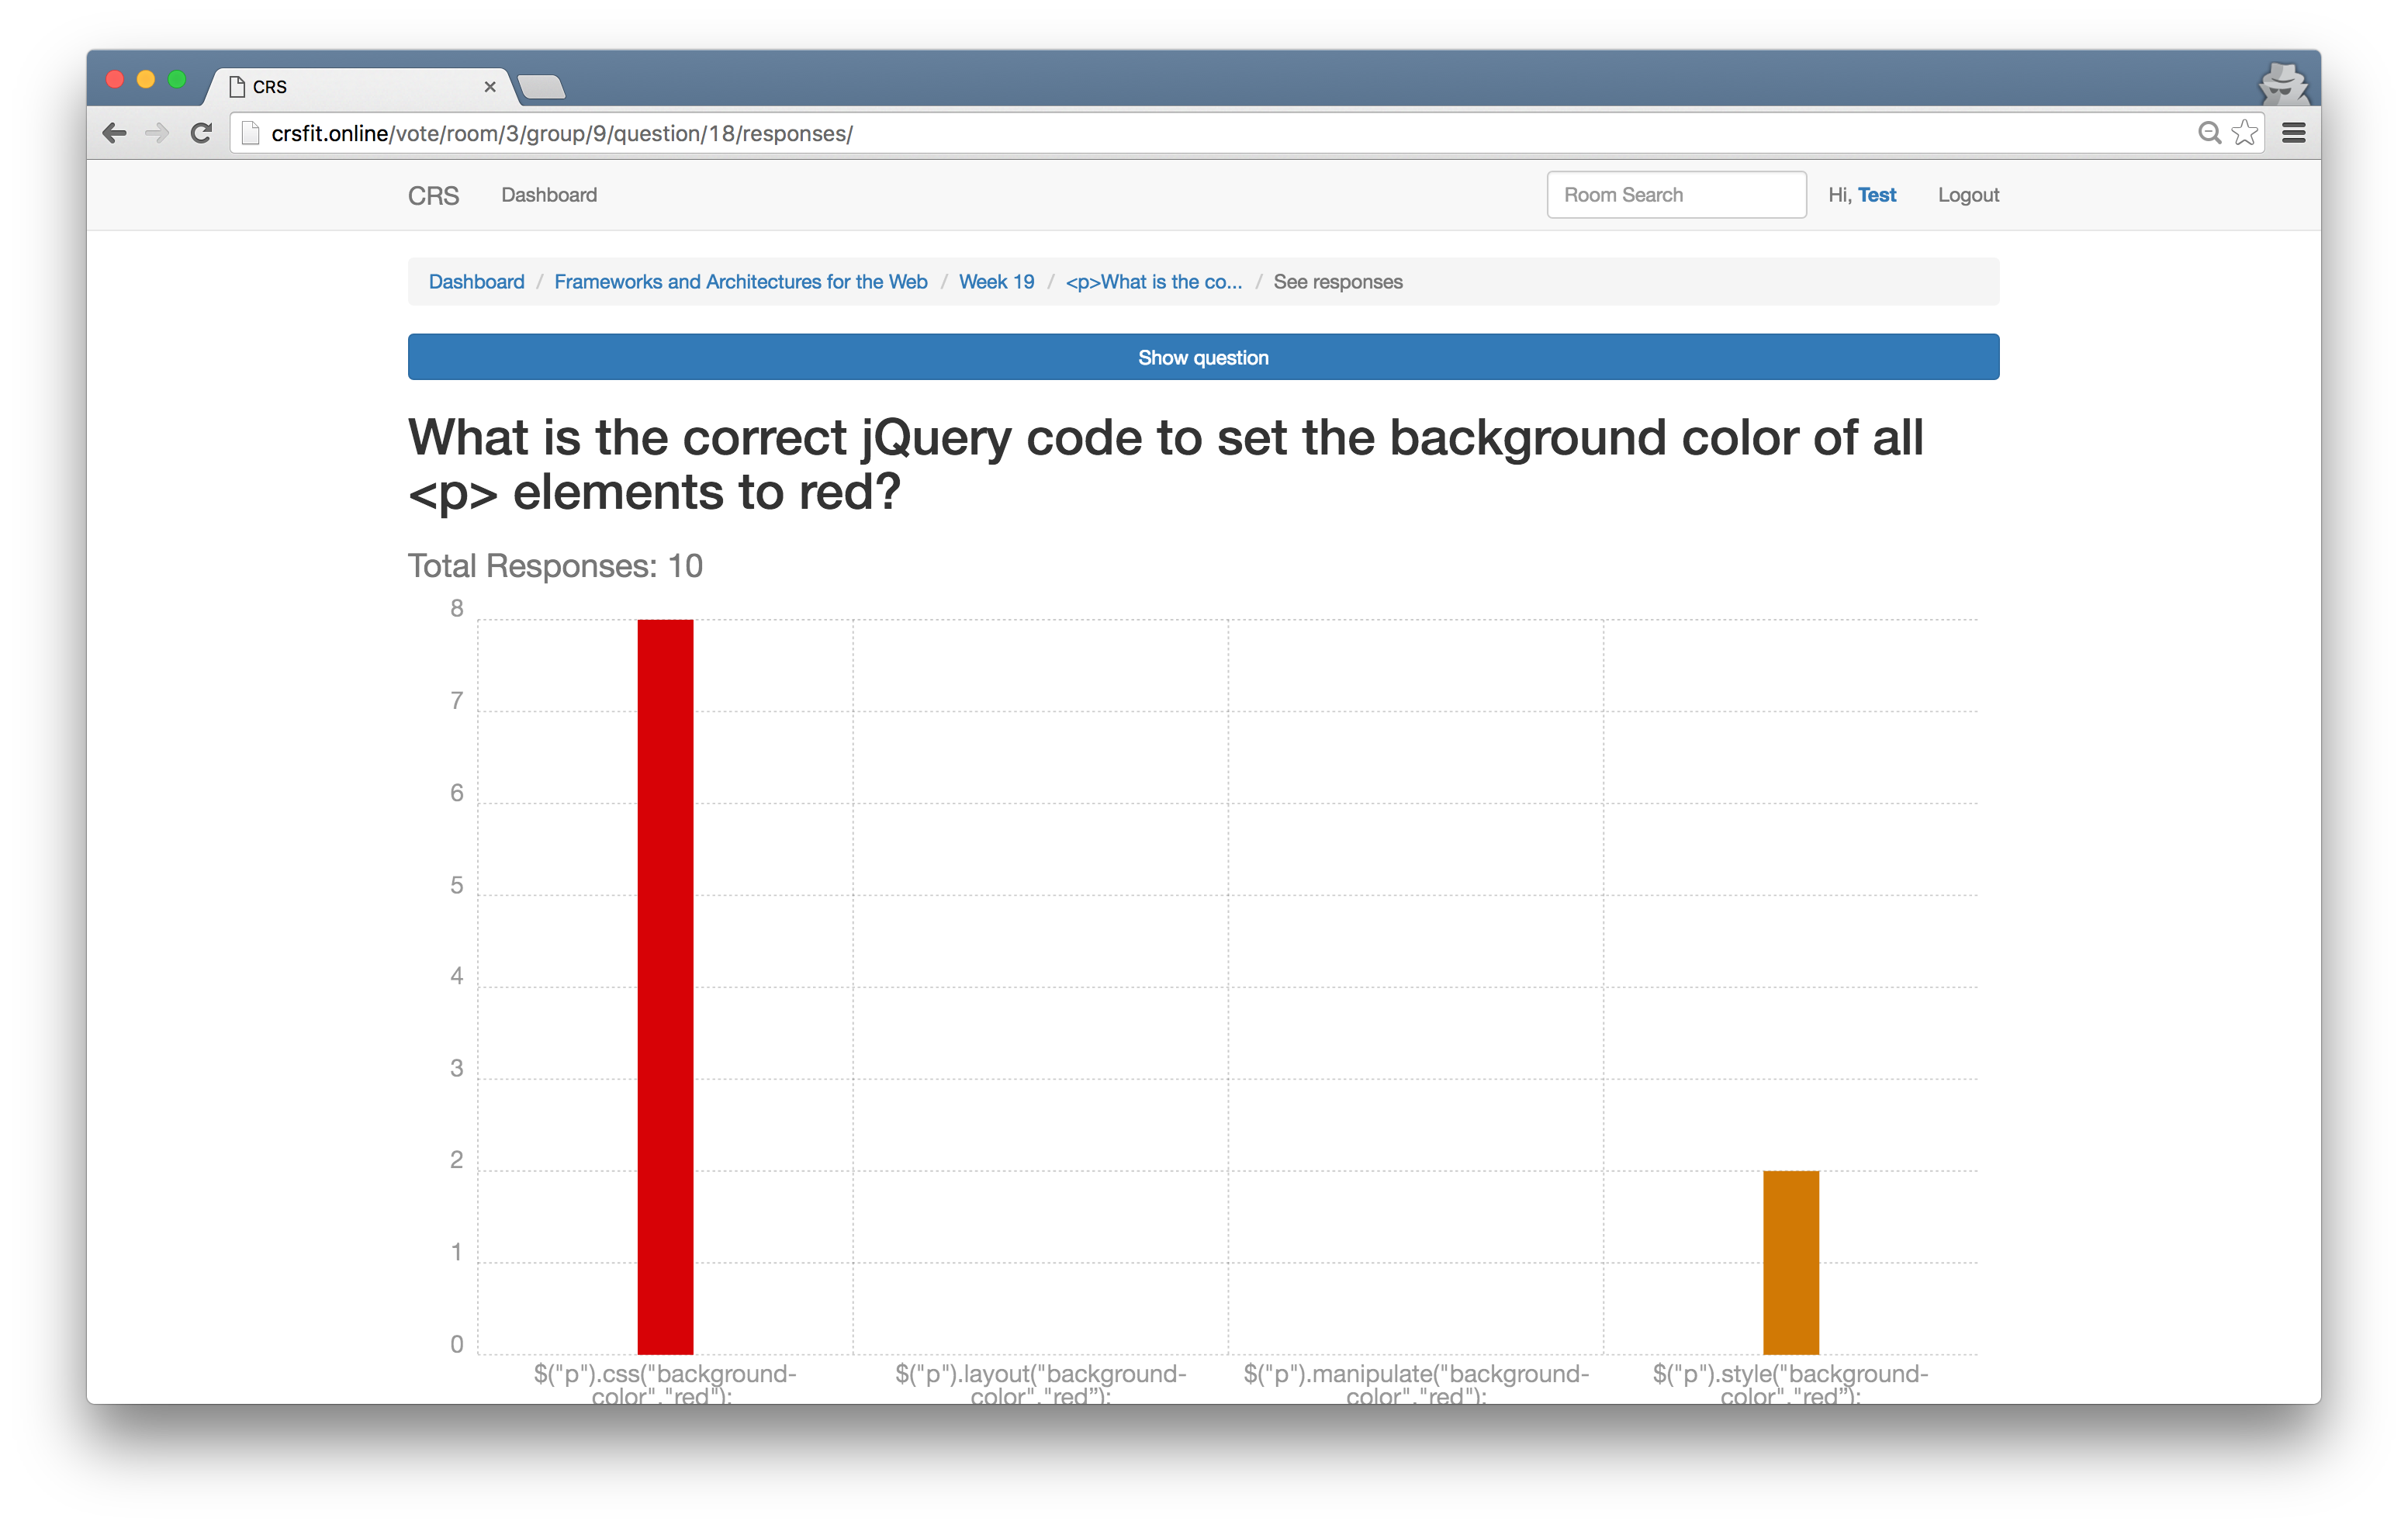
\includegraphics[width=\textwidth]{responses.png}
	\caption[The response page]{A view of the page with live updated responses in a chart.}\label{fig:responses}
\end{figure}

When students are answering a question they see a screen like in figure \ref{fig:question}. Here they are able to select and submit an answer.

\begin{figure}[H]
\capstart
	\centering
		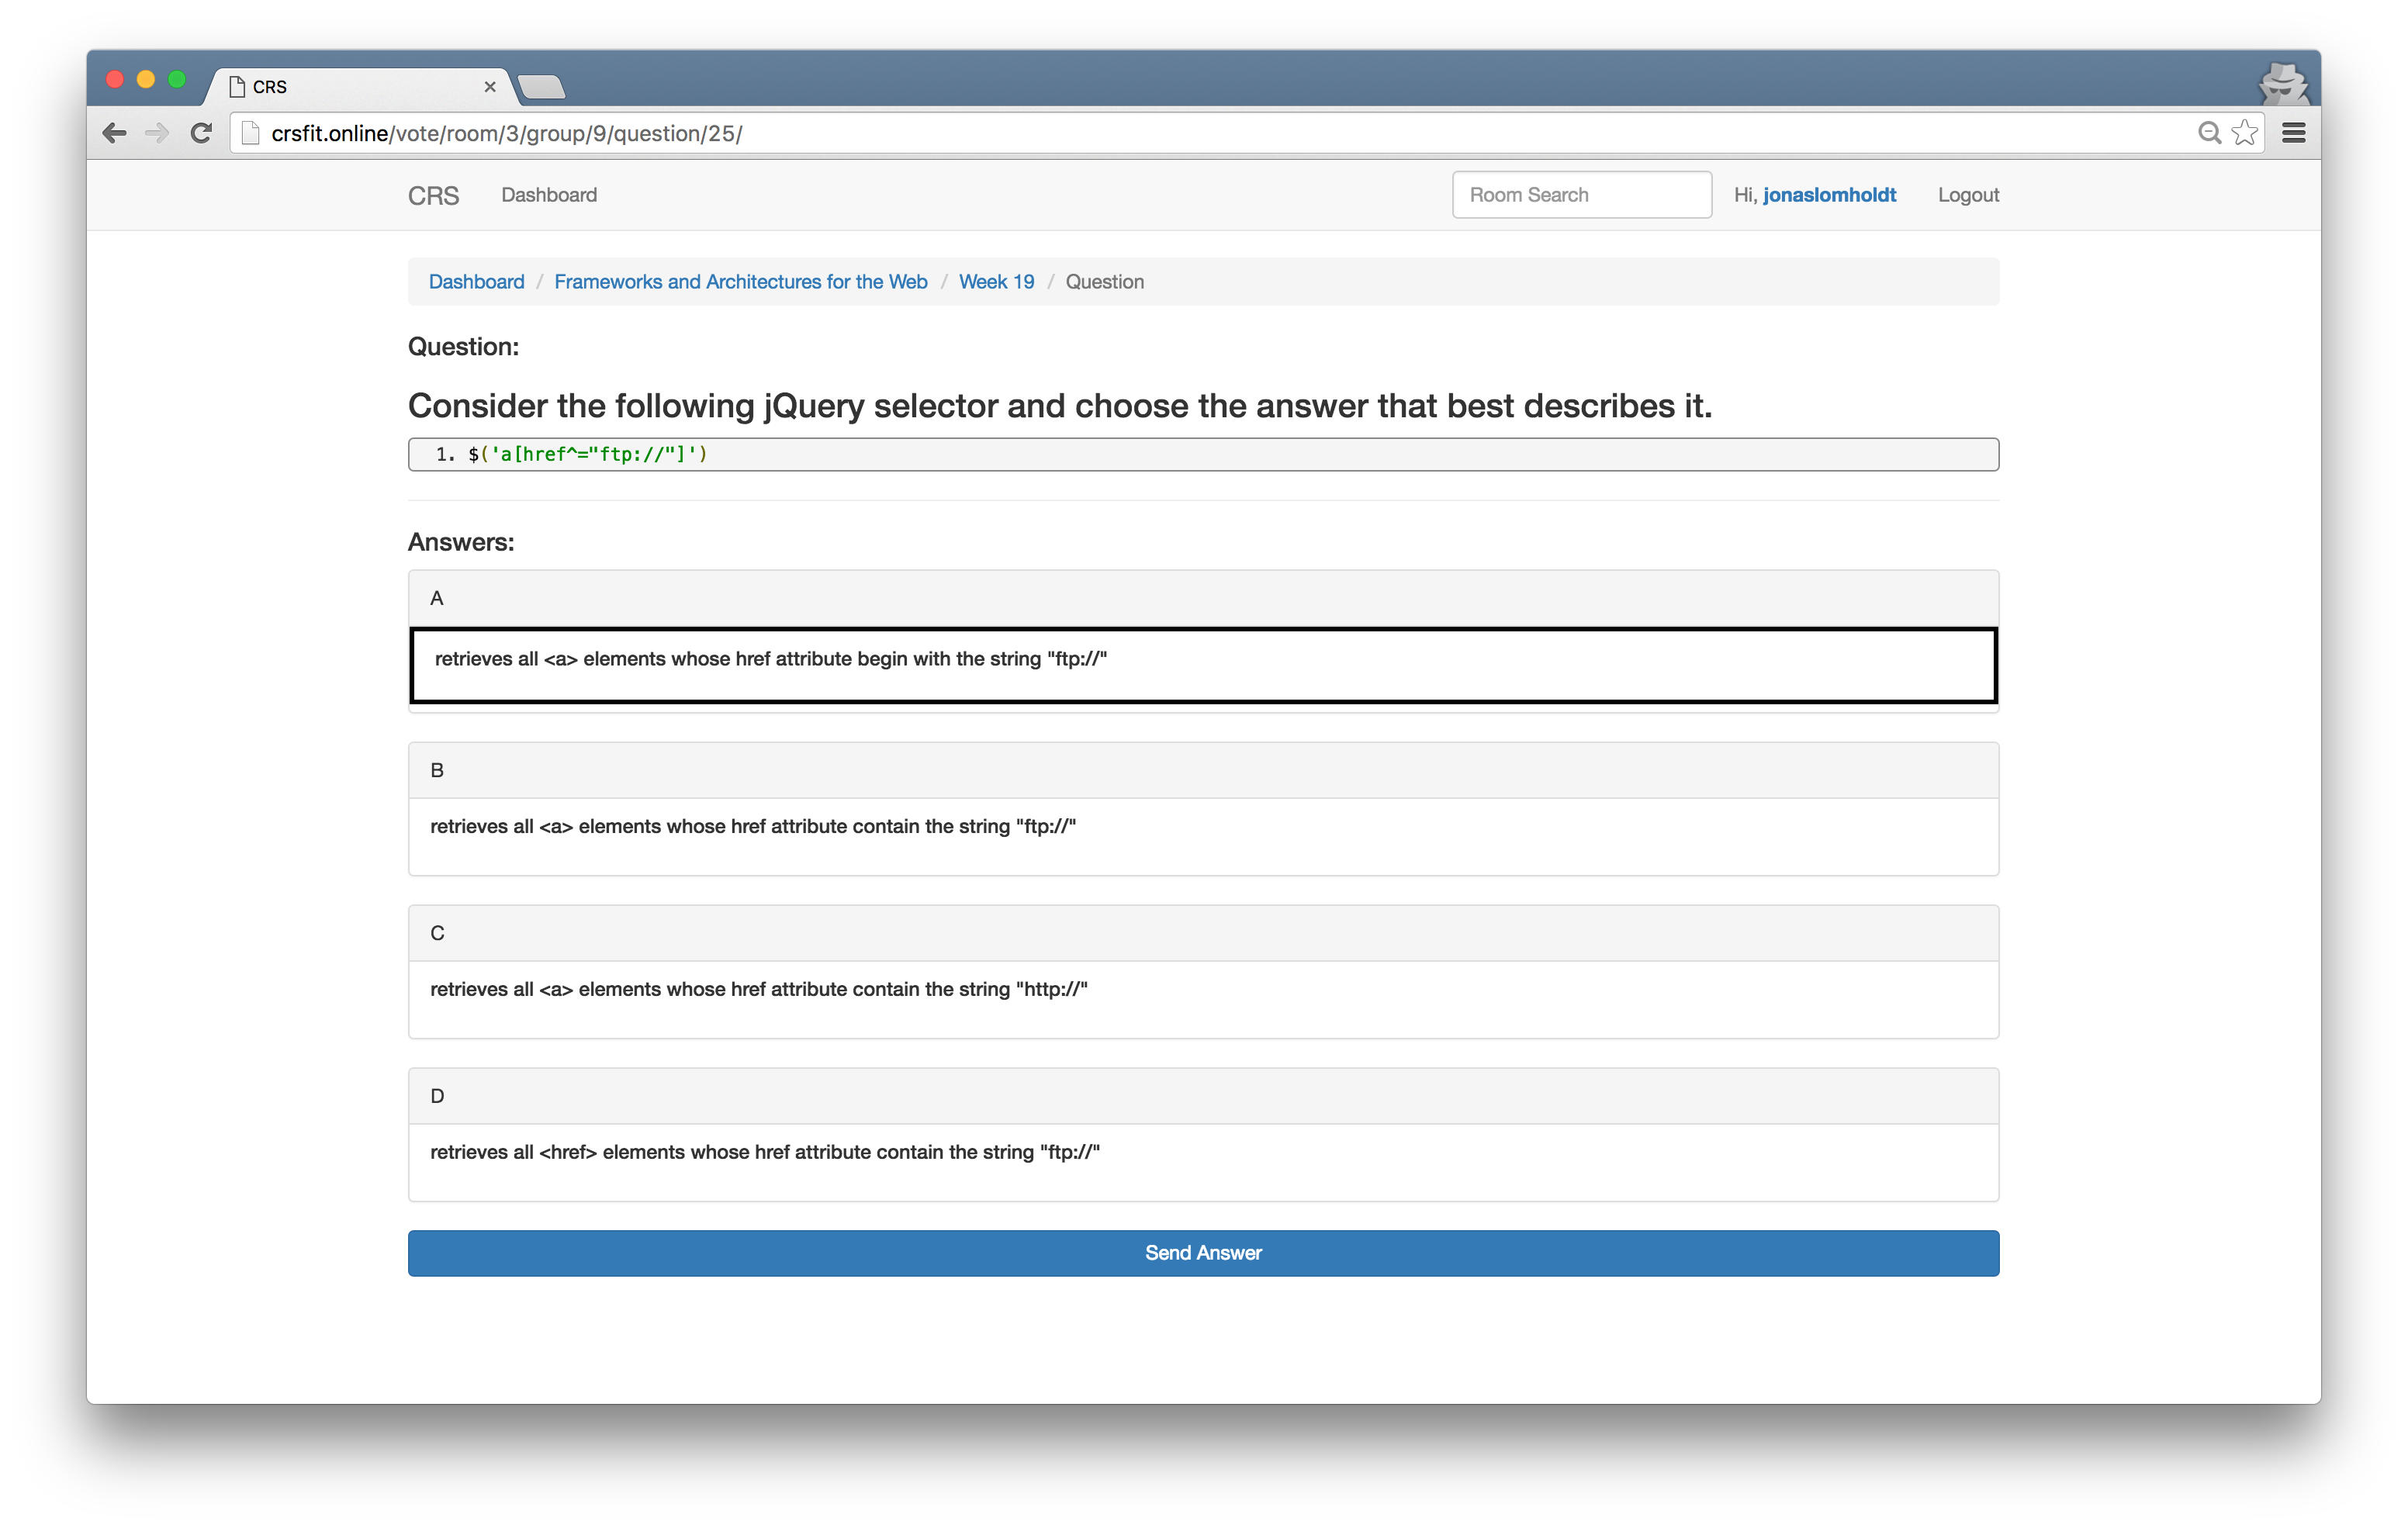
\includegraphics[width=\textwidth]{question.png}
	\caption[A question page]{View of a question with four answering options.}\label{fig:question}
\end{figure}

The system includes features which are not described in this section. That's features that are not essential for the system to work as we intend, but features we found suitable or nice to have during the development of CRSFIT. The technical description of the system will include more details which will include mentions of some of these features.